
% NOTE: necessary when ptmx or no mathfont class option is given
% \providecommand{\upGamma}{\Gamma}
% \providecommand{\uppi}{\pi}
\appendices
% \begin{appendices}
\section{Single Deep Neural Network}
\label{dnn_app}
A Deep Neural Network (DNN) is a computational network that can be considered as a function $\mathcal{M}_\Theta:~\mathcal{D} \rightarrow \hat{Y}$ in which $\mathcal{D}$ is a set of input data fed into the network, $\Theta$ is a set of network parameters (weights and biases), and $\hat{Y}$ is the output set of the approximated values $\hat{y} \in \hat{Y}$. Moreover, the DNN model $\mathcal{M}_{\Theta}$ aims to be trained based on its input data (a finite set of training data) denoted by $\mathcal{D}$, according to the function~$\mathcal{Q}:~\mathcal{D}~\rightarrow~Y$ such that, 
\[
\mathcal{Q} = \{\ (d_{i},y_{i})\ |\ i \in \mathbb{N}^{[1,m]}\ \}\ ,
\]
where $i$ is a data point with $d_{i}$ and $y_{i}$ representing features and target labels, respectively and $m$ is the number of participating data points (data samples) in the training dataset.

In the DNN model $\mathcal{M}_{\Theta}$, we intend to optimize a loss function in the form of $\mathcal{L}(\mathcal{D},\Theta;Y)$. This optimization is performed by minimizing the average of each data sample $i$'s loss value with respect to the parameter set of $\Theta$ defined as, 
\begin{equation}
\min_{\Theta}\ \mathcal{L}(\mathcal{D},\Theta;Y) = \frac{1}{m}\ \sum_{i=1}^{m} loss(d_{i},\Theta;y_{i})\ ,
\label{loss}
\end{equation}
where $loss(d_{i},\Theta;y_{i})$ is the loss function of the single data sample $i$ in the training dataset.

\section{Opinion Determinants in Subjective Logic}
\label{sl_app}
\vspace{.2cm}
\noindent\textbf{Definition 1 (Belief and Disbelief Masses).} The belief $b$ and disbelief $d$ are the amount of being in support of and against the truth of a particular subjective variable in a DNN provided by a DNN component, respectively~\cite{sl}. % $\hfill \blacksquare$

\vspace{.2cm}
\noindent\textbf{Definition 2 (Uncertainty Mass).} The uncertainty $u$ is the amount of not being confident (certain) or not having sharp idea regarding the truth of a subjective variable provided by a DNN component. The uncertainty is caused by vacuity of evidence in a DNN model. Thus, the fewer observations (data samples) may give rise to more uncertainty~\cite{sl}.% $\hfill \blacksquare$

\vspace{.2cm}
\noindent\textbf{Definition 3 (Base Rate Mass).} The base rate $a$ is the prior probability for a subjective variable that can be interpreted as a kind of bias term which provided by a DNN component. The base rate can help us take the bias measure into account~\cite{sl}. % $\hfill \blacksquare$

{\color{red} \section{Parameter Opinion Initialization}
\label{parint_app}
We initialize the model parameters opinions according to the lack (vacuity) of observations by Uncertainty Maximization~\cite{sl} on randomly generated opinions from uniform distribution $\mathcal{U}(0,1)$ with respect to the opinion additivity requirement~\ref{additivity}. In Uncertainty Maximization, an opinion for the parameter $\theta$ should have at least one belief mass of zero, i.e. $b_{\theta} = 0$ and the uncertainty is calculated as,
\begin{equation}
    u_{\theta} = \min(1,\frac{PP_{\theta}}{a_{\theta}})\ ,
\end{equation}
where $PP_{\theta}$ and $a_{\theta}$ is the projected probability and the base rate of the parameter $\theta$'s opinion, respectively.}

{\color{red}
\section{Parameters Opinion Update}
\label{opt_app}
To optimize the total opinion of our model (minimizing the uncertainty while maximizing the belief), we need to update the parameters' opinions based on the error value $|y-\hat{y}|$ that the model is achieving during training. Thus, we exploit back propagation approach for the parameters' opinion updates while we are updating the actual parameters in mini-batch gradient descent to minimize the loss function. Based on what we perform in back propagation process to update the parameters in each layer, we initialize the opinions of parameters' change, $O_{\Delta w}$ and $O_{\Delta b}$, backward from the last layer towards the first layer using error opinion set $O_{\delta}$ and its pairwise multiplication with predicted opinion set $O_{\hat{y}}$ in the previous layer. For instance, in layer $i$,
\begin{equation}
    O_{\Delta b}^i = O_{\delta} \qquad \textnormal{and} \qquad O_{\Delta w}^i = O_{\delta} \otimes O_{\hat{y}}^{i-1}\ .
\end{equation}

Finally, in each layer $i$ with the neuron set $layer_i$, we update the error opinion set $O_{\delta}$ by assigning a set consists of multi-source average fusion on the pairwise multiplication of the previous $O_{\delta}$ and the weight opinion set $O_{w}^i$ as follows:
\begin{equation}
    O_{\delta} = \{ \bigoplus_{layer_i}(O_{\delta}\ \otimes\ O_{w}^i)\ \}\ .
\end{equation}

Then, we update the opinion of each parameter $\theta$ denoted by $O_{\theta}$, by taking cumulative fusion on its previous opinion and its change opinion denoted by $O_{\Delta \theta}$, as follows:
\begin{equation}
    O_{\theta} = O_{\theta}\ \widehat{\oplus}\ O_{\Delta \theta}\ .
\end{equation}
}

{\color{red}
\section{Impact of Data Distribution on Model Performance}
\label{impact_app}
The objective of this preliminary experiment is to demonstrate how the distributional properties in input data can impact the model performance. We used Pima Indians Diabetes Dataset\footnote{\url{https://www.kaggle.com/datasets/uciml/pima-indians-diabetes-database}} originally from the National Institute of Diabetes and Digestive and Kidney Diseases. 

We apply classification task using different traditional classifiers like K-nearest, Logistic Regression, Random Forest, AdaBoost, and a DNN classifier (\emph{MLPClassifier} with three layers optimized by Adam and with initial learning rate of 0.01) on both original distributions (e.g. skewed) and transformed distributions (e.g., no longer skewed). 
%K-nearest, Logistic Regression, Random Forest, AdaBoost, and Bagging classifiers on the original and transformed data features. 
%For the DNN classifier, we used \emph{MLPClassifier} as a three-layer neural network model optimized by Adam and initial learning rate of 0.01. 
As shown in Figure~\ref{skew_dist}, the distribution of the three most skewed features of the dataset named \emph{Insulin}, \emph{DiabetesPedigreeFunction}, and \emph{Age} as well as the transformed features are shown. Therefore, in Figure~\ref{skew_acc}, we can see the accuracy of different classifiers including the DNN model over the original and transformed distributions of the most skewed features that hold the highest skewness and kurtosis in this dataset.
\begin{figure}[!ht]  % H
	\centering
	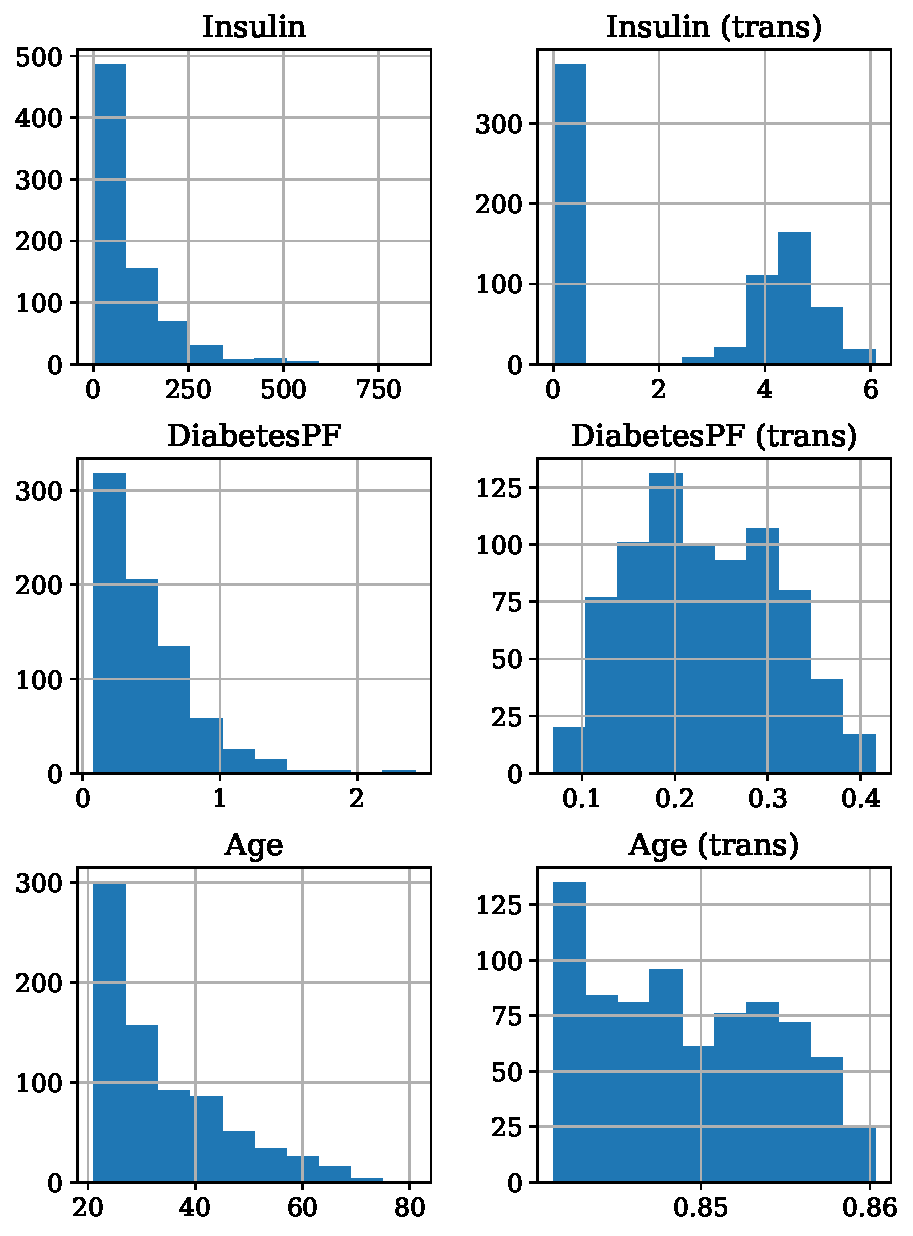
\includegraphics[width=0.4\textwidth]{figures/dist.pdf}
	\vspace{-0.3cm}
	\caption{The original and transformed distributions of the three most skewed features of the Pima Indians Diabetes Dataset}
%	\label{skew_dist}
\end{figure}
\begin{figure}[!ht]  % H
	\centering
	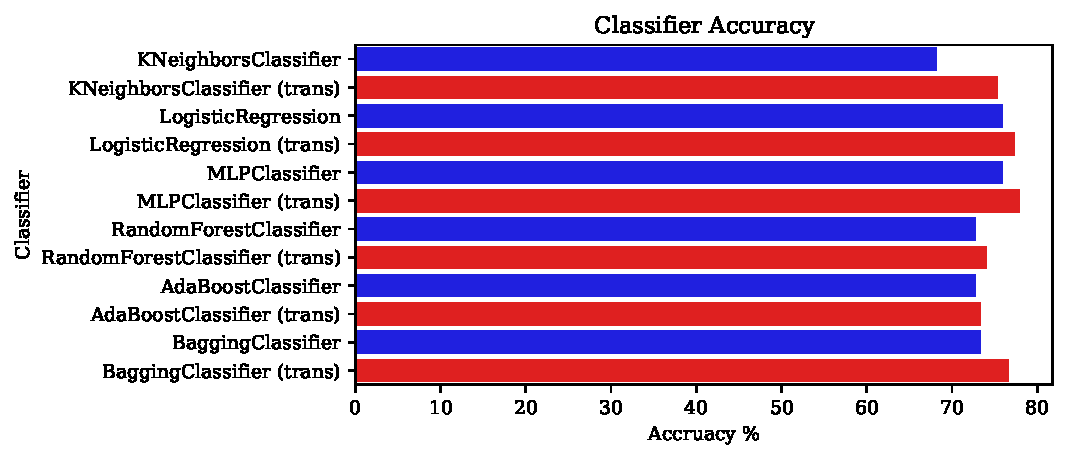
\includegraphics[width=0.5\textwidth]{figures/classifiers.pdf}
	\vspace{-0.7cm}
	\caption{The model accuracy of different classifiers based on the original (green bars) and transformed (red bars) distributions of the three most skewed features of the Pima Indians Diabetes Dataset}
%	\label{skew_acc}
\end{figure}
The results show that the transformed feature distribution mitigates the skewness and kurtosis as two distributional properties of training data. We can see the accuracy improvement of all classifiers in the presence of transformed features. Therefore, the skewed training data features, that have higher kurtosis as well, can negatively impact the DNN performance. This result also indicates the necessity of considering statistical and distributional properties of input data in initializing data opinions before propagation through the DNN network. 
}

{\color{red}
\section{Model Training}
\label{train_app}
Figures~\ref{susy_loss} and~\ref{kdd_loss} illustrate that the training process over both SUSY and KDD Cup 99 datasets has been performed effectively for both datasets as decreasing loss and increasing accuracy during the training process shown in these figures is a sign of a successful learning process. 
\begin{figure}[ht]  % H
	\centering
% 	\vspace{-10cm}
	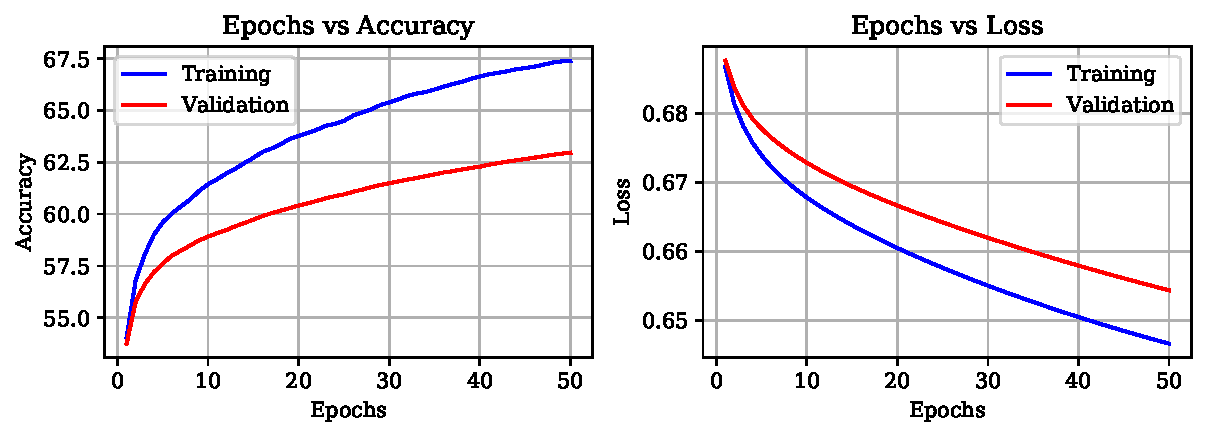
\includegraphics[width=0.5\textwidth]{figures/Results_susy.pdf}
	\vspace{-0.3cm}
	\caption{The accuracy and loss values during 45 training epochs over SUSY dataset}
%	\label{susy_loss}
\end{figure}
\begin{figure}[ht] % H
\centering
% \vspace{-22cm}
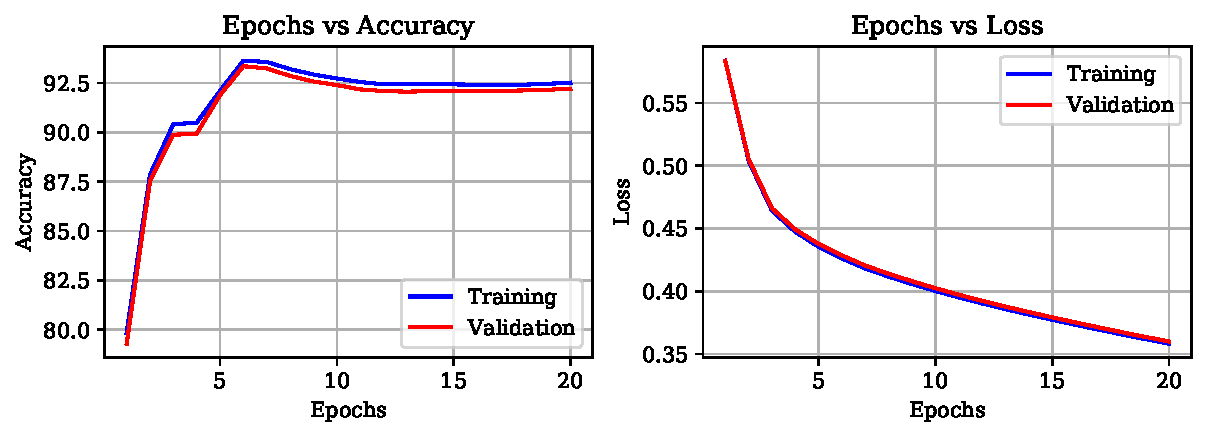
\includegraphics[width=0.5\textwidth]{figures/Results_kdd.pdf}
\vspace{-0.3cm}
\caption{The accuracy and loss values during 20 training epochs over KDD Cup 99 dataset}
%\label{kdd_loss}
\end{figure}
}

\section{Investigation on Optimal Thresholds in Opinion Optimization}
\label{thr_app}

{\color{blue} According to Equation~\ref{makeop}, in the opinion optimization process, we use two different thresholds $\phi_1$ and $\phi_2$ to determine the error opinion $O_\delta^l$ for each target label $l$. Thus, we need to find the optimal values for selecting the thresholds. In this regard, we applied the proposed method using Susy dataset on different selections of the thresholds with respect to their requirements mentioned in Section~\ref{op_opt}. Figure~\ref{susy_thr} shows the model opinion results during training using different selections of the two thresholds. We can observe that when $\phi_1=0.4$ and $\phi_2=0.7$ (the purple line), we see the higher amount of model belief and trustworthiness along with lower amount of disbelief rather than other choices of thresholds.
}
\begin{figure*}[t]  % H
	\centering % width=\textwidth
	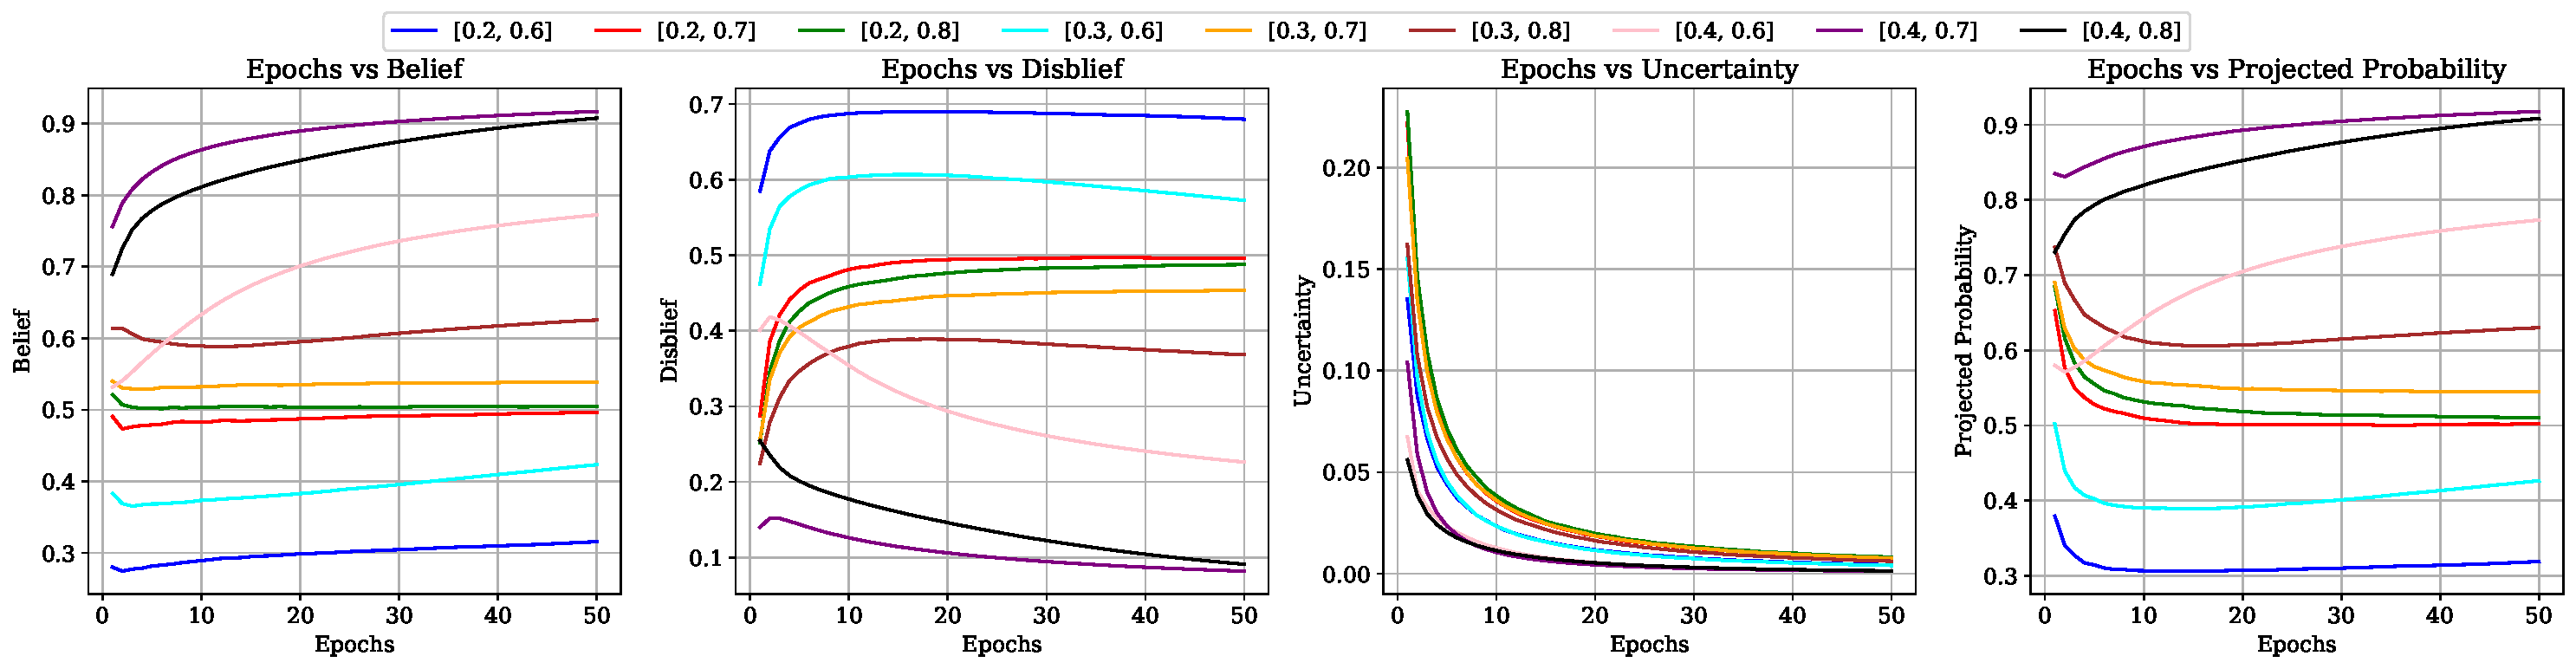
\includegraphics[width=0.8\textwidth]{figures/Results_susy_thr.pdf}
	\vspace{-0.3cm}
	\caption{The behavior of each determinant of total model opinion with respect to different selections of opinion optimization thresholds $\phi_1$ and $\phi_2$}
	\label{susy_thr}
\end{figure*}
%\begin{figure*}[!ht]
%	\centering % width=\textwidth
%%	\includegraphics[width=0.8\textwidth]{figures/Results_kdd_thr.pdf}
%	\vspace{-0.3cm}
%	\caption{The improvement process of opinion determinants during 20 training epochs based on different factors in numerical features over KDD Cup 99 dataset}
%	\label{kdd_thr}
%\end{figure*}


%%%%%%%%%%%%%%%%%%%%%%%%%%%%%%%%%%%%%%%%%%%%%%%%%%%%%%%%%%%%%%%

% \section{Subjective Logic}
% \label{sl_app}
% In the following, the required definitions and concepts in subjective logic are provided: 

% \noindent\textbf{Definition 1 (Belief and Disbelief Masses):} The belief $b_v$ and disbelief $d_v$ are the amount of being in support of and against the truth of a particular subjective variable in a DNN provided by the DNN component $v$, respectively. $\hfill \blacksquare$

% \noindent\textbf{Definition 2 (Uncertainty Mass):} The uncertainty $u_v$ is the amount of not being confident (certain) or not having sharp idea regarding the truth of a subjective variable provided by the DNN component $v$. $\hfill \blacksquare$

% \noindent\textbf{Definition 3 (Base Rate Mass):} The base rate $a_v$ is the prior probability for a subjective variable that can be interpreted as a kind of bias term which provided by the DNN component $v$. $\hfill \blacksquare$

% The base rate can help us take the bias measure into account which is beneficial for different settings like federated learning to analyze the impact of fairness in private data on the total opinion of a model.

% \noindent\textbf{Definition 4 (Binomial Opinion):} An opinion about a subjective variable $x$ in a binary domain $\mathbb{X}=\{x,\overline{x}\}$ is a \emph{Binomial Opinion} owned by a DNN component. A binomial opinion~\cite{sl} by the DNN component $v$ about the model performance as the subjective variable, is defined as a tuple, $\hfill \blacksquare$
% \begin{equation}
%     O_{v} = \{b_{v},d_{v},u_{v},a_{v}\} \quad \text{s.t.} \quad b_v,d_v,u_v,a_v \in \mathbb{R}^{[0, 1]}\ ,
% \label{op}
% \end{equation}
% where $b_v$ denotes the amount of belief in support of the subjective variable $x$, $d_v$ denotes the amount of disbelief about $x$, the uncertainty mass $u_v$ represents the lack of confidence about $x$ caused by vacuity of evidence in a DNN model, and $a_v$ is the prior probability about $x$ without considering any evidence which can take a prior bias measure into account. Furthermore, these opinion masses should meet the following additivity requirement: 
% \begin{equation}
% b_v + d_v + u_v = 1
% \label{additivity}
% \end{equation}

% A binomial opinion by the DNN component $v$ is equivalent to a Beta PDF which is a particular binary version of Dirichlet PDF. The expected probability of the PDF yields to a projected probability as trustworthiness of a DNN component which considers the component's belief and uncertainty about model performance simultaneously as,
% % Therefore, a bijective mapping between a binomial opinion and a Beta PDF is defined as the equality between the expected probability of a Beta PDF and the projected probability of a binomial opinion~\cite{sl}. Therefore, this expectation can yield to a projected probability as trustworthiness of a DNN model which is considering the model belief and uncertainty about model performance simultaneously as, 
% \begin{equation}
%     \text{Projected Probability:} \quad PP_v = b_v + u_v.a_v
% \label{projprob}
% \end{equation}

% Therefore, we exploit subjective logic to generate opinions of an imaginary agent or a DNN component about a subjective variable like model performance in a neural network setting. % In this paper, the subjective variable is accuracy or generally, the model performance.

% The propagation process of different components' opinions through a DNN will be performed with the help of specific attributes of opinions, e.g., fusion and multiplication) with respect to its impact on the particular parameter.
% Furthermore, there are some important operators defined in subjective logic to calculate the output opinion achieved based on the specific relations amongst two or more opinions as operands. The opinion operators and relations amongst opinions are either binary~\cite{sl} or multi-source operators~\cite{multi1}. In the following, we exploit the operators for opinion computation based on particular concepts and interpretations. These opinion operators are Multiplication ($\otimes$), Comultiplication ($\widehat{\otimes}$), Average Fusion ($\oplus$), and Multi-source Average Fusion ($\bigoplus$). 
% and Multi-source Weighted Fusion ($\widehat{\bigoplus}$).
% In the following, we discuss our proposed methodology on uncertainty propagation and the procedure of data opinion initialization in detail.

%%%%%%%%%%%%%%%%%%%%%%%%%%%%%%%%%%%%%%%%%%%%%%%%%%%%%%%%%%%%%%%%%%%%%%%%%%%%%%%%%%%%%%%%%%%%%%%%%%%%%%%%%

% \noindent\textbf{Definition 4 (Binomial Opinion):} Let $x$ be the only subjective variable, and a binary domain specified as $\mathbb{X}~=~\{x,\overline{x}\}$ consisting of the subjective variable $x$ and its complement $\overline{x}$. Thus, an opinion about a binary random variable $x \in \mathbb{X}$ is a \emph{Binomial Opinion} owned by a DNN component. A binomial opinion by the DNN component $v$ in our learning system about the performance of our DNN in the training round $t$ is defined as a tuple,
% \[
%     O_{v} = \{b_{v},d_{v},u_{v},a_{v}\} \quad \text{s.t.} \quad b_v,d_v,u_v,a_v \in \mathbb{R}^{[0, 1]}\ \ \hspace{1cm}  \blacksquare
% \]

% In the Definition 4, $b_v$ denotes the amount of belief in support of the subjective variable $x$, $d_v$ denotes the amount of disbelief about $x$, the uncertainty mass $u_v$ represents the lack of confidence about $x$ caused by vacuity of evidence in a DNN model, and $a_v$ is the prior probability about $x$ without considering any evidence. Furthermore, these opinion masses should meet the following additivity requirement: 
% \[
% b_v + d_v + u_v = 1
% \]

% \[
% \textit{Opinion} = \{\textit{Belief},\ \textit{Disbelief},\ \textit{Uncertainty},\ \textit{Base Rate}\}
% \] 

% \begin{equation}
% \omega_v = \{ b_v,\ d_v,\ u_v,\ a_v \}
% \label{opinion}
% \end{equation}

% In this research, each DNN component $v$ in $\mathcal{M}_{\Theta}^t$ has a binomial opinion about the subjective concept $x$ which is the model's performance (accuracy) since each specific DNN component can be impacted by the DNN model performance in each training epoch.

% A binomial opinion by a model's component $v$ is equivalent to a Beta PDF which is a particular binary version of Dirichlet PDF. Therefore, a bijective mapping between a binomial opinion and a Beta PDF is defined as the equality between the expected probability of a Beta PDF and the projected probability of a binomial opinion~\cite{sl}. Therefore, this expectation can yield to a projected probability which is considering the belief and uncertainty about a subjective variable simultaneously as follows: 
% \begin{equation}
%     \text{Projected Probability:} \quad PP_v = b_v + u_v.a_v
% \label{projprob}
% \end{equation}

% Moreover, the \emph{Degree of Conflict} (DC)~\cite{sl} is a measure of the opinion difference between two different DNN components $v$ and $v'$ which is defined as, 
% \begin{equation}
%     DC_{vv'}^t = PD_{vv'}^t.CC_{vv'}^t\ ,
% \label{DC_eq}
% \end{equation}
% \text{where}
% \[
% \text{Projected Difference:} \quad PD_{vv'}^t = |PP_v^t - PP_{v'}^t|\ ,
% \]
% % \text{and}
% \[
% \text{Conjunctive Certainty:} \quad CC_{vv'}^t = (1-u_v^t).(1-u_{v'}^t)\ .
% \]

% Since both $PD_{vv'}^t, CC_{vv'}^t \in [0,1]$, then $DC_{vv'}^t \in [0,1]$. DC exploits belief and uncertainty in clients' opinions about a subjective variable which here is the model performance. 

%%%%%%%%%%%%%%%%%%%%%%%%%%%%%%%%%%%%%%%%%%%%%%%%%%%%%%%%%%%%%%%

% \section{Parameter Opinion Initialization}
% \label{par_op_init}
% After initializing the inputs' opinions (feature opinions), we are going to optimize (or minimize) the loss function using Gradient Descent (GD). However, we utilized a modified version of batch GD which uses parameters' opinions instead of parameters' values. In~\cite{hope}, Even though the authors proposed a brief computation procedure on how to calculate neuron opinions through the layers in a DNN, the paper do not describe the detailed computation on the parameters' initialization, update rules, and back-propagation procedure.
% \begin{algorithm}[!h]  %tbh - H - ht - !htbp
% \DontPrintSemicolon
% \SetInd{0.2em}{1.3em} %Moved vertical bar to the left, default is 0.5 and 1.0
% \SetAlgoLined
% % \SetAlgoNoLine
%   \vspace{1mm}
%   \KwInput{\\ \vspace{1mm} $\mathcal{M}$: The neural network model;\\
%   \vspace{1mm} $\Theta_\mathcal{M}$: The parameter set of the model $\mathcal{M}$;}
%   \vspace{1mm}
%   \KwOutput{\\ \vspace{1mm} $O_\Theta^{\mathcal{M}}$: The parameter opinions for the model~$\mathcal{M}$;} 
%     \vspace{2mm}
%     $O_\Theta^{\mathcal{M}} \leftarrow \emptyset$   \tcp*{Parameter ops}
%     \vspace{1mm}
%     \For{\textnormal{each parameter} $\theta \in \Theta_\mathcal{M}$}
%     {
%     \vspace{1mm}
%     $a_{\theta} \leftarrow $ A random real number from $\mathcal{N}(0.5,{\varepsilon}^2)$ \;
%     \vspace{1mm}
%     $b_{\theta}, d_{\theta}, u_{\theta} \leftarrow $ Random real numbers from $\mathcal{U}(0,1)$ \;
%     \vspace{1mm}
%     $b_{\theta}, d_{\theta}, u_{\theta} \leftarrow$ \textit{softmax}($b_{\theta}, d_{\theta}, u_{\theta}$) \;
%     % \vspace{1mm}
%     % $PP_{\theta} \leftarrow b_{\theta} + a_{\theta}.u_{\theta}$ \;
%     \vspace{1mm}
%     \tcp{Uncertainty Maximization}
%     $b_{\theta} \leftarrow 0$ \;
%     \vspace{1mm}
%     $u_{\theta} \leftarrow \min(1,\frac{PP_{\theta}}{a_{\theta}})$ \;
%     \vspace{1mm}
%     $d_{\theta} \leftarrow 1 - u_{\theta}$ \;
%     \vspace{1mm}
%     Adding $O_\theta^{\mathcal{M}}$ to $O_\Theta^{\mathcal{M}}$ \;
%     }
%     \Return{$O_\Theta^{\mathcal{M}}$}
% \caption{Parameter Opinion Initialization}
% \label{algo2}
% \end{algorithm}

% Therefore, we need to firstly initialize the parameters' opinions (opinions for weights and biases) in our model $\mathcal{M}$ before the first training epoch. In the Algorithm~\ref{algo2}, we utilize \emph{Uncertainty Maximization} approach which is described in~\cite{sl} to maximize the amount of uncertainty to initialize a parameter's opinion. However, we do not assign a vacuous opinion to the parameters as $u=1$ since it can be interpreted as a biased operation which is far from randomization. Therefore, we need to uniformly assign random values from $\mathcal{U}(0,1)$ with respect to the subjective logic rule~\ref{additivity} as additivity requirement. In Uncertainty Maximization, an opinion (for the parameter $\theta$) should have at least one belief mass of zero and the uncertainty is calculated as,
% \begin{equation}
%     u_{\theta} = \min(1,\frac{PP_{\theta}}{a_{\theta}})\ ,
% \end{equation}
% where $PP_{\theta}$ and $a_{\theta}$ is the projected probability and the base rate of the parameter $\theta$'s opinion, respectively.

%%%%%%%%%%%%%%%%%%%%%%%%%%%%%%%%%%%%%%%%%%%%%%%%%%%%%%%%%%%%%%%

% \section{Feed Forward Opinion Propagation}
% \label{feed_op}
% After opinion initialization of the parameters in the DNN model $\mathcal{M}$, we need to define an approach based on what is proposed in~\cite{hope} for forward propagation of opinions in our model; however, we had to slightly change it here. As the Algorithm~\ref{algo3} indicates, we utilize comultiplication between weight opinions and input opinions of neurons in each layer. Then, we do average fusion on these results for each neuron including the neuron's bias opinion to generate each neuron's total opinion. 

% As it is stated in~\cite{sl}, the reason for using comultiplication between weight and input opinions in each layer is to consider the existence (presence) of at least one of them in the process of feed forwarding. In addition, we use average fusion on the opinion results because these opinions observe each neuron simultaneously (the same process over the same time period). Thus, each neuron's opinion is dependent to the opinion of weights and the previous layer's neurons.
% \begin{algorithm}[!h]  %tbh - H - ht - !htbp
% \DontPrintSemicolon
% \SetInd{0.2em}{1.3em} %Moved vertical bar to the left, default is 0.5 and 1.0
% \SetAlgoLined
% % \SetAlgoNoLine
%   \vspace{1mm}
%   \KwInput{\\ \vspace{1mm} $O_x^F$: The opinions of batch of input data for the feature set $F$; \\
%   \vspace{1mm} $O_{\Theta}^{\mathcal{M}}$: The parameter opinions for the model~$\mathcal{M}$; }
%   \vspace{1mm}
%   \KwOutput{\\ \vspace{1mm} $O_{\hat{y}}$: The output (predicted) opinions for the model~$\mathcal{M}$;}
%     \vspace{2mm}
%     $O_{\hat{y}} \leftarrow O_x^F$ \;
%     \vspace{1mm}
%     \For{\textnormal{each layer $i$ in the model} $\mathcal{M}$}
%     {
%     \vspace{1mm}
%     $O_n^i \leftarrow \emptyset$ \tcp*{Each layer ops}
%     \vspace{1mm}
%     \For{\textnormal{each neuron $j$ in the layer $i$}}
%     {
%     \vspace{1mm}
%     $O_{list}^j \leftarrow \emptyset$ \;
%     \vspace{1mm}
%     Adding $O_{\hat{y}}\; \widehat{\otimes}\; O_w^{i,j}$ to $O_{list}^j$ \;
%     \vspace{1mm}
%     Adding $O_b^j$ to $O_{list}^j$ \;
%     \vspace{1mm}
%     Adding $\bigoplus(O_{list}^j)$ to $O_n^i$ \;
%     }
%     \vspace{1mm}
%     $O_{\hat{y}} \leftarrow O_n^i$ \;
%     }
%     \Return{$O_{\hat{y}}$}
% \caption{Forward Opinion Propagation in the DNN Model $\mathcal{M}$}
% \label{algo3}
% \end{algorithm}
% After feed forwarding the opinions of input data through the network which is already initialized by the input data, we need to optimize the parameters' opinion based on the loss function and the gradient descent approach which is completely indicated in the Algorithm~\ref{algo4}. It means that we are going to exploit back propagation approach to minimize the amount of uncertainty and maximize the amount of belief in the total opinion of our model $\mathcal{M}$. According to the fact that the number of neurons in the output layer is as same as the number of labels (classes) in the target (in classification tasks), the total opinion of our neural network model $\mathcal{M}$ is calculated by applying multi-source average fusion over the output opinions of output (last) layer's neurons $l \in L$ as follows:
% \begin{equation}
%     O_{\mathcal{M}} = \bigoplus_{l \in L}(O_{out}^l)
% \end{equation}

%%%%%%%%%%%%%%%%%%%%%%%%%%%%%%%%%%%%%%%%%%%%%%%%%%%%%%%%%%%%%%%

% \section{Parameter Opinion Optimization Algorithm}
% \label{par_opt}

% \begin{algorithm}[h!]  %tbh - H - ht - !htbp
% \DontPrintSemicolon
% \SetInd{0.2em}{1.3em} % Moved vertical bar to the left, default is 0.5 and 1.0
% \SetAlgoLined
% % \SetAlgoNoLine
%   \vspace{1mm}
%   \KwInput{\\ \vspace{1mm} $\mathcal{D}_b$: Batch of training data $\mathcal{D}$ in size $b$; \\
%   \vspace{1mm} $P_y^b$ and $P_{\hat{y}}^b$: The actual and predicted output which are $b \times n_l$ matrices for the data batch $\mathcal{D}_b$;\\
%   \vspace{1mm} $n_{\mathcal{M}}$: Total number of layers in the DNN model $\mathcal{M}_\Theta$; \\
% %   \vspace{1mm} $T$: Total number of required training rounds; \\ \vspace{1mm} $C_t$: Finite set of participating clients at the training round~$t$;
%   }
%   \vspace{1mm}
%   \KwOutput{\\ \vspace{1mm} $O_{\mathcal{M}}$: The total opinion for the DNN model~$\mathcal{M}_\Theta$;}
%     \vspace{2mm}
%     \For{\textnormal{each batch} $\mathcal{D}_b$ \textnormal{of the training data} $\mathcal{D}$}
%     {
%     \vspace{1mm}
%     $O_{out}, O_{\delta} \leftarrow \emptyset$ \tcp*{output and error ops}
%     \vspace{1mm}
%     $O_x^F, O_y^L \leftarrow$ \textit{init\_op}($\mathcal{D}_b, y_b$) \tcp*{Algo.~\ref{algo1}}
%     \vspace{1mm}
%     $O_{\hat{y}}^L \leftarrow$ \textit{forward\_op}($O_x^F,O_\Theta^{\mathcal{M}}$) \tcp*{Algo.~\ref{algo3}}
%     \vspace{1mm}
%     $\Delta_b^L \leftarrow |P_{\hat{y}}^b - P_y^b|$ \tcp*{$b \times n_l$ matrix}
%     \vspace{1mm}
%     \For{\textnormal{each label} $l \in L$}
%     {
%     \vspace{1mm}
%     $r_b^l, s_b^l, w_b^l \leftarrow$ Number of evidence in $\Delta_b^l \subset \Delta_b^L$ over $(0:\phi_1:\phi_2:1)$ \;
%     \vspace{1mm}
%     $O_e^l \leftarrow$ \textit{make\_op}($r_b^l, s_b^l, w_b^l$) \tcp*{Eq.~\ref{makeop}}
%     \vspace{1mm}
%     $O_{back}^l \leftarrow$ $O_e^l\; \widehat{\otimes}\; O_y^l$ \;
%     \vspace{1mm}
%     Adding $O_{back}^l\; \oplus\; O_{\hat{y}}^l$ to $O_{out}$\;
%     \vspace{1mm}
%     Adding $O_e^l$ to $O_{\delta}$\;
%     }
%     \vspace{1mm}
%     \For{\textnormal{all neurons in the layer} $i=n_{\mathcal{M}}$ \textnormal{to} $1$}
%     {
%     \vspace{1mm}
%     $O_{\Delta b}^i \leftarrow O_{\delta}$ and $O_{\Delta w}^i \leftarrow$ $O_{\delta} \otimes O_{\hat{y}}^{i-1}$ \;
%     \vspace{1mm}
%     $O_{b}^i \leftarrow$ $O_{b}^i \oplus O_{\Delta b}^i$ and $O_{w}^i \leftarrow$ $O_{w}^i \oplus O_{\Delta w}^i$\; 
%     \vspace{1mm}
%     $O_{temp} \leftarrow \emptyset$ \;
%     \vspace{1mm}
%     \For{\textnormal{each neuron in the layer} $i-1$}
%     {
%     $O_{list}^{i-1} \leftarrow \emptyset$ \;
%     \vspace{1mm}
%     \For{\textnormal{each neuron in the layer} $i$}
%     {
%     \vspace{1mm}
%     Adding $O_{\delta}\; \widehat{\otimes}\; O_{w}^i$\ to\ $O_{list}^{i-1}$\;
%     }
%     \vspace{1mm}
%     Adding $\bigoplus(O_{list}^{i-1})$ to $O_{temp}$ \;
%     }
%     \vspace{1mm}
%     $O_{\delta} \leftarrow O_{temp}$ \;
%     }
%     }
%     \vspace{1mm}
%     $O_{\mathcal{M}} \leftarrow$ $\bigoplus(O_{out})$ \tcp*{Average Fusion}
%     \textbf{end} \;
%     \Return{$O_{\mathcal{M}}$}
% \caption{Opinion Optimization Based on Loss Function Using Back Propagation Approach}
% \label{algo4}
% \end{algorithm}

% \end{appendices}










